\subsection{Client Connection}
\label{sub:eval:connection}

\begin{figure*}
    \minipage{0.32\textwidth}%
        \centering
        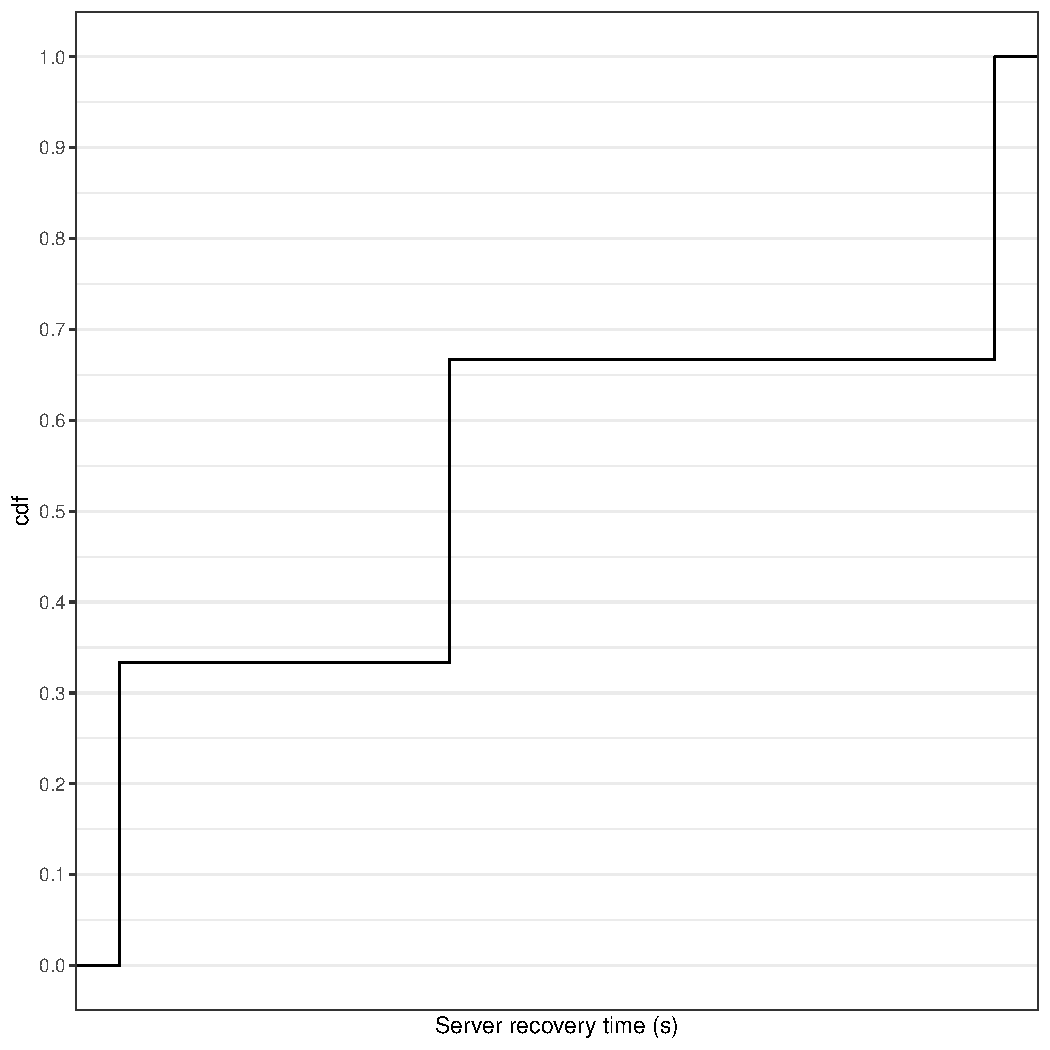
\includegraphics[width=0.9\linewidth]{server-recovery}
        \caption{Recovery time after a server failure}\label{fig:server-recovery}%
    \endminipage\hfill
    \minipage{0.32\textwidth}
        \centering
        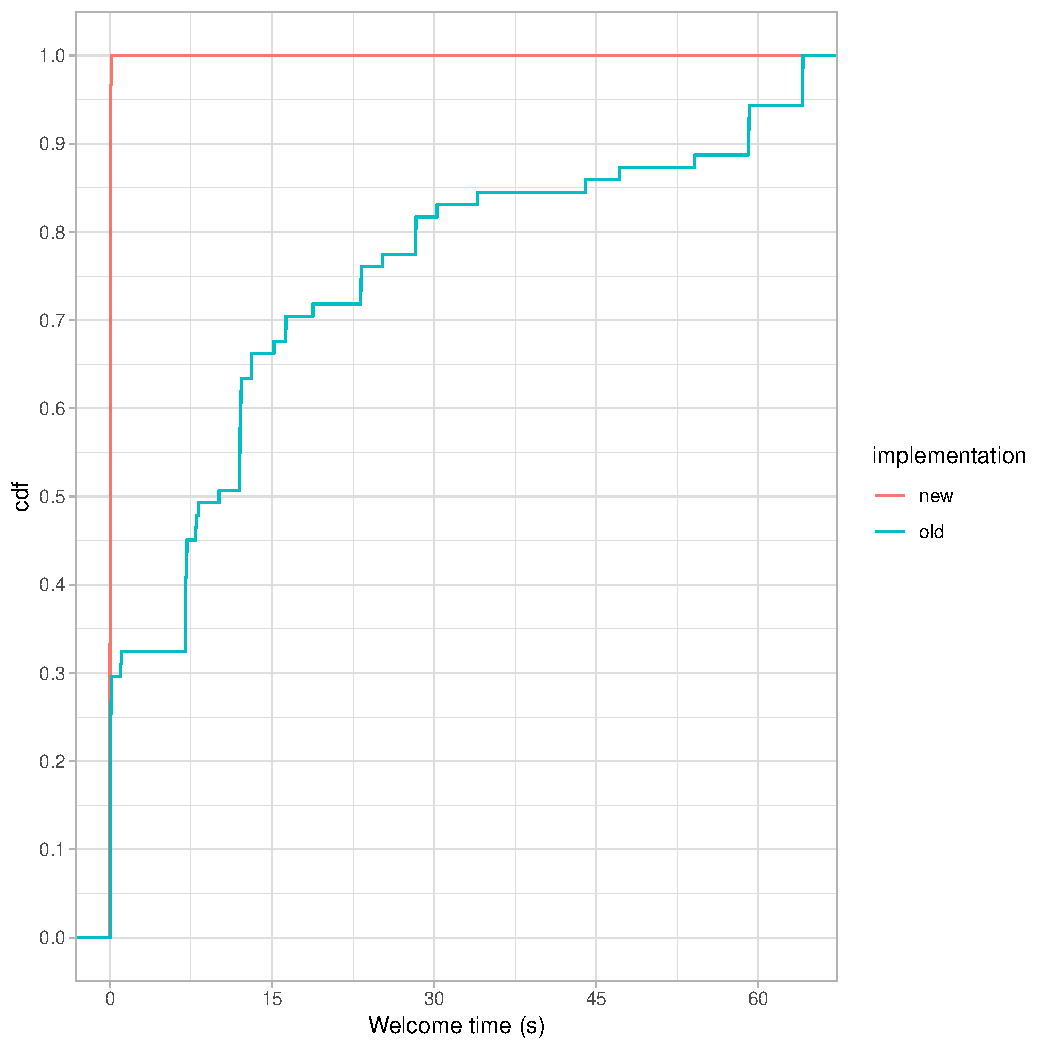
\includegraphics[width=0.89\textwidth]{client-welcome}
        \caption{Client connection time until receiving a copy of the state}\label{fig:client-welcome}%
    \endminipage\hfill
    \minipage{0.32\textwidth}
        \centering
        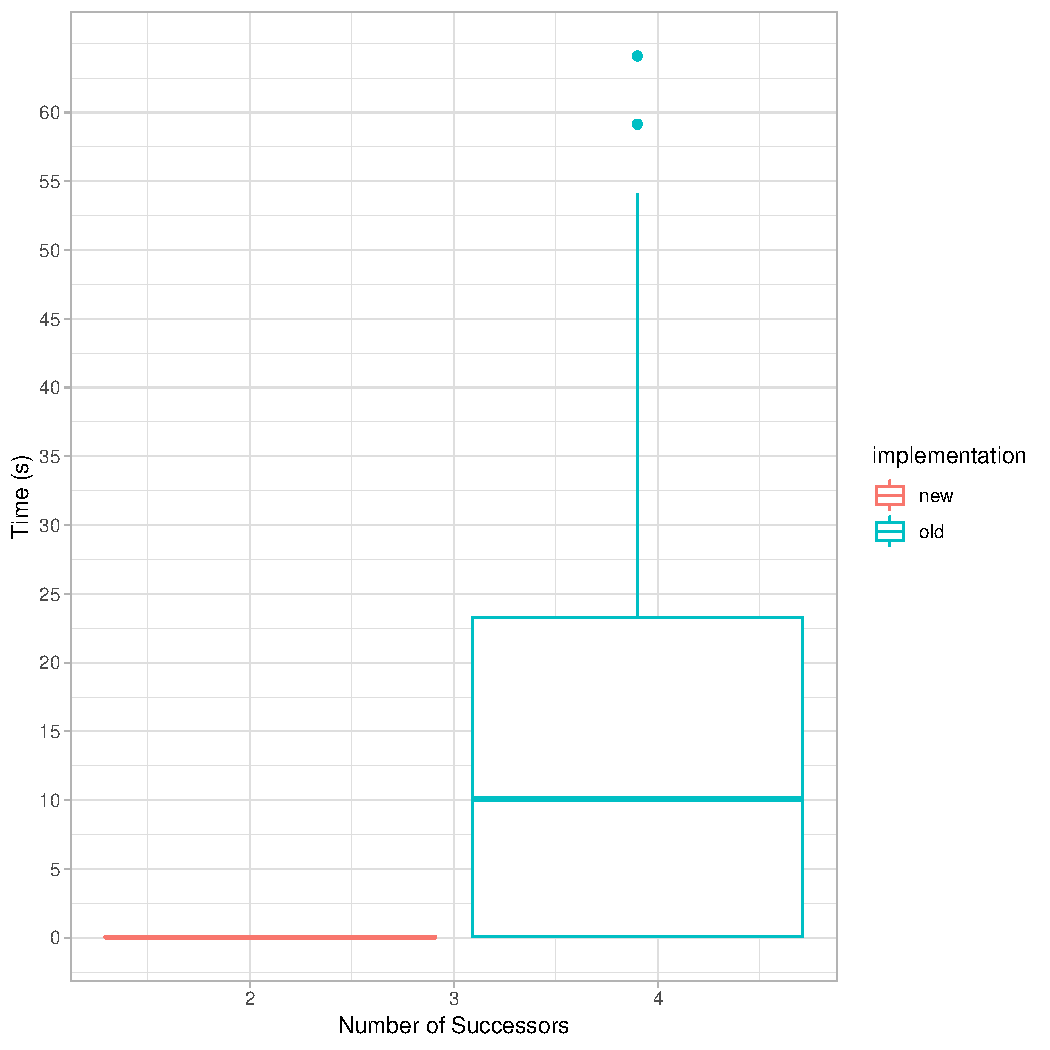
\includegraphics[width=0.9\textwidth]{client-welcome-successors}
        \caption{Client time to connect per number of successors}\label{fig:client-welcome-successors}%
    \endminipage\hfill
\end{figure*}

We define client connection as the amount of time it takes for a device to connect to a published server as a client. 
This takes into account not only the time it takes for a client to connect to the server, but also the time it takes for a client to own its copy of the server state. 
Events related to client connection were used for this measurement, namely \texttt{welcome} messages sent from the server in the handshake and the first \texttt{stateupdate} event received at the client.

Figure~\ref{fig:client-welcome} presents the cumulative empirical function for client connection.
On average, clients are fully connected to a published server in 11 seconds ($\rpm$ 16 seconds). 
The majority of the clients (80\%) were able to establish a connection under 15 seconds, 
but we noticed some cases were clients took longer to connect. 
Inspecting these edge cases, we identified that these were mostly related with scenarios were the state was larger than 1MB. 
In other cases were this affirmation did not hold, we hypothesize that the mobile network connection was not stable, but we lack data to support this hypothesis.

In order to further investigate client connection properties, we analyzed whether the number of connected devices or the server state size may influence connection time.
Figure~\ref{fig:client-welcome-successors} presents a boxplot chart for the connection time grouped by the number of successors. 
Despite the fact that all connected clients received a state update with the most recent \texttt{successors} list, 
we could not see how the number of successors would influence a new client connection and all boxplot charts overlap.

On the other hand, Figure~\ref{fig:client-welcome-state-size} models time as a linear function of the server state size.
Intuitively, as the server state increases in size, clients take longer to connect. 
This give us insights about benefits and limitations of our current implementation.
Based on client connection measurements, we posit that \APIshort could scale with more connect devices, though the state variable is a bottleneck and applications that require a larger state are compromised.